\section{Introduction: one object, two descriptions}\label{sec:intro}

\subsection{A familiar situation}

Much of the mathematics a student learns in the first three years consists of describing the same object in two ways and comparing the descriptions.

\begin{itemize}
\item A linear map $u : \mathbb R^n\to\mathbb R^n$ can be described by its matrix in a basis. The matrix depends on the basis; the map does not. A property of $u$ that does not depend on the basis, such as \q{$u$ is invertible}, can be read on any matrix of $u$: $\det A\neq 0$. Reading it on two matrices $A$ and $P^{-1}AP$ of the same map gives the theorem $\det A\neq 0\iff\det(P^{-1}AP)\neq 0$, which is not hard, but which we would not have looked for without the map in the middle.
\item A finite abelian group can be described by generators and relations, or by its invariant factors. The number of its elements of order dividing~$2$ is an invariant; computing it in both descriptions gives an identity between them.
\item A closed surface can be described by a triangulation or by a cell decomposition. The Euler characteristic $V-E+F$ is an invariant; computing it in both descriptions gives the same number, and that equality is a theorem about the two combinatorial objects.
\end{itemize}

In each case there is an object (the linear map, the group, the surface), two \emph{presentations} of it, and an \emph{invariant}: a property or a quantity attached to the object, which we know how to read on each presentation. The two readings must agree, and that agreement is a statement about the presentations alone, in which the object no longer appears.

\subsection{Caramello's bridges}

Olivia Caramello has shown that this pattern is especially fruitful when the object in the middle is a \emph{Grothendieck topos} \cite{caramello-unification,caramello-tst}. A topos, which we shall introduce gently in \S\ref{sec:shapes}--\S\ref{sec:sites}, is a category that behaves like the category of sets, and that can be presented in a great many ways: by a small category, by a \q{site}, or as the classifying topos of a logical theory. Two presentations that look nothing alike can give the same topos; and many properties of a topos (being Boolean, being De Morgan, having enough points, being connected, \dots) have a concrete meaning on each presentation. Caramello calls the resulting pattern a \emph{bridge}:
\begin{center}
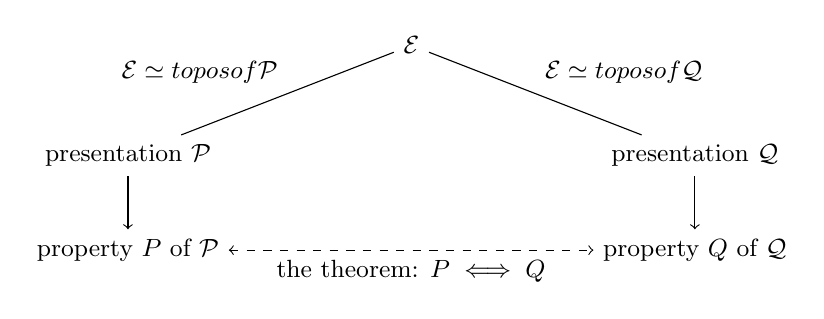
\begin{tikzpicture}[every node/.style={font=\small}]
\node (E) at (0,1.4) {$\mathcal E$};
\node (P) at (-3.6,0) {presentation $\mathcal P$};
\node (Q) at (3.6,0) {presentation $\mathcal Q$};
\node (a) at (-3.6,-1.2) {property $P$ of $\mathcal P$};
\node (b) at (3.6,-1.2) {property $Q$ of $\mathcal Q$};
\draw (P) -- node[above left]{$\mathcal E\simeq\text{topos of }\mathcal P$} (E);
\draw (Q) -- node[above right]{$\mathcal E\simeq\text{topos of }\mathcal Q$} (E);
\draw[dashed,<->] (a) -- node[below]{the theorem: $P\iff Q$} (b);
\draw[->] (P) -- (a);
\draw[->] (Q) -- (b);
\end{tikzpicture}
\end{center}
The equivalence of topoi in the middle is the \emph{deck} of the bridge; the two characterisations of the invariant, one on each side, are its \emph{arches}. Once a deck and an invariant are chosen, the theorem $P\iff Q$ follows mechanically.

\subsection{Theorems generated automatically}

In a talk at Mines Paris in September 2024, Caramello proposed to turn this into a program \cite{caramello-mines}. A proof assistant would take as inputs \q{a database of topos equivalences} and \q{a database of characterizations of topos-theoretic invariants in terms of different presentations for toposes}, and would combine the decks with the arches \q{to generate concrete correspondences between `unravelings' of a given invariant in terms of different presentations for a given topos} \cite[slide 11]{caramello-mines}. She warns that the results \q{can be rather `weird' according to the usual mathematical standards}, but that \q{with a careful choice of topos equivalences and invariants, one can easily get interesting and natural mathematical results} \cite[slide 8]{caramello-mines}. The talk also lists the work this requires: formalising topos theory in the proof assistant Lean, building the two databases, and rewriting machine output into statements a human can read.

\subsection{What this text does}

This text is an experiment in that direction, small enough to be done by hand and to be read by a third-year student.

\begin{enumerate}
\item We introduce, with examples, the few notions needed: small categories seen as \q{shapes}, presheaves as \q{structures of that shape}, subobjects and their negation, the Ore condition, idempotents (\S\ref{sec:shapes}--\S\ref{sec:same}). Sites and classifying topoi get a lighter treatment (\S\ref{sec:sites}).
\item We state five bridges (the \emph{arches}), which are proved in Lean~4 in the library \lp{} of lean-pool. Two of them we prove in full, with elementary means, because the proofs are short and instructive (\S\ref{sec:arches}).
\item We assemble a small database of \emph{decks}: structures that a student meets under other names, and which turn out to be presheaves on some small category (\S\ref{sec:generator}).
\item We run the generator: each deck combined with each arch gives a statement. We write each statement in elementary terms, explain how the generator finds it, prove it again directly without any topos theory, give examples, and say whether we found it in the literature (\S\ref{sec:monoids}--\S\ref{sec:theories}).
\end{enumerate}

The outputs range from the classical to the (as far as we can tell) unstated. Among the latter, three readings may amuse a computer scientist: for deterministic automata over an alphabet with at least two letters, the weak law of excluded middle fails, while it holds for one letter (\S\ref{sec:monoids}); for an abstract rewriting system, the same law holds in the associated topos exactly when the system is confluent in the sense of Church and Rosser (\S\ref{sec:preorders}); and the \q{fibre functors} of the monoid of $n\times n$ matrices are counted by the possible ranks, $n+1$ of them (\S\ref{sec:points}).

\subsection{What this text does not claim}

None of the generated statements is deep. Each has a direct proof of a few lines, and we give it: that is the point. A theorem generator does not need to produce hard theorems to be useful; it needs to produce \emph{correct} statements that someone would not have thought of formulating, in a form that can then be checked. The direct proofs are our check. We have searched the literature for each statement (\S\ref{sec:lit}), and most of them are in print, often in the work of Johnstone, Caramello, Hemelaer and Rogers, which is what one should expect when a generator is run on the simplest decks. Where we did not find a statement, we say so, and we would welcome a reference.

\subsection{How to read this text}

\S\ref{sec:shapes}--\S\ref{sec:arches} are the course: read them in order. \S\ref{sec:same} and \S\ref{sec:sites} can be skimmed on a first reading; they are needed for \S\ref{sec:points} and \S\ref{sec:theories}. \S\ref{sec:monoids}--\S\ref{sec:theories} can then be read in any order. Exercises are scattered through the text; hints and solutions are in \S\ref{sec:solutions}. Prerequisites: groups, rings, linear algebra, a first course in topology (open and closed sets), and the definition of a category and a functor (which we recall).
